% Options for packages loaded elsewhere
\PassOptionsToPackage{unicode}{hyperref}
\PassOptionsToPackage{hyphens}{url}
\documentclass[
]{article}
\usepackage{xcolor}
\usepackage[margin=1in]{geometry}
\usepackage{amsmath,amssymb}
\setcounter{secnumdepth}{-\maxdimen} % remove section numbering
\usepackage{iftex}
\ifPDFTeX
  \usepackage[T1]{fontenc}
  \usepackage[utf8]{inputenc}
  \usepackage{textcomp} % provide euro and other symbols
\else % if luatex or xetex
  \usepackage{unicode-math} % this also loads fontspec
  \defaultfontfeatures{Scale=MatchLowercase}
  \defaultfontfeatures[\rmfamily]{Ligatures=TeX,Scale=1}
\fi
\usepackage{lmodern}
\ifPDFTeX\else
  % xetex/luatex font selection
\fi
% Use upquote if available, for straight quotes in verbatim environments
\IfFileExists{upquote.sty}{\usepackage{upquote}}{}
\IfFileExists{microtype.sty}{% use microtype if available
  \usepackage[]{microtype}
  \UseMicrotypeSet[protrusion]{basicmath} % disable protrusion for tt fonts
}{}
\makeatletter
\@ifundefined{KOMAClassName}{% if non-KOMA class
  \IfFileExists{parskip.sty}{%
    \usepackage{parskip}
  }{% else
    \setlength{\parindent}{0pt}
    \setlength{\parskip}{6pt plus 2pt minus 1pt}}
}{% if KOMA class
  \KOMAoptions{parskip=half}}
\makeatother
\usepackage{color}
\usepackage{fancyvrb}
\newcommand{\VerbBar}{|}
\newcommand{\VERB}{\Verb[commandchars=\\\{\}]}
\DefineVerbatimEnvironment{Highlighting}{Verbatim}{commandchars=\\\{\}}
% Add ',fontsize=\small' for more characters per line
\usepackage{framed}
\definecolor{shadecolor}{RGB}{248,248,248}
\newenvironment{Shaded}{\begin{snugshade}}{\end{snugshade}}
\newcommand{\AlertTok}[1]{\textcolor[rgb]{0.94,0.16,0.16}{#1}}
\newcommand{\AnnotationTok}[1]{\textcolor[rgb]{0.56,0.35,0.01}{\textbf{\textit{#1}}}}
\newcommand{\AttributeTok}[1]{\textcolor[rgb]{0.13,0.29,0.53}{#1}}
\newcommand{\BaseNTok}[1]{\textcolor[rgb]{0.00,0.00,0.81}{#1}}
\newcommand{\BuiltInTok}[1]{#1}
\newcommand{\CharTok}[1]{\textcolor[rgb]{0.31,0.60,0.02}{#1}}
\newcommand{\CommentTok}[1]{\textcolor[rgb]{0.56,0.35,0.01}{\textit{#1}}}
\newcommand{\CommentVarTok}[1]{\textcolor[rgb]{0.56,0.35,0.01}{\textbf{\textit{#1}}}}
\newcommand{\ConstantTok}[1]{\textcolor[rgb]{0.56,0.35,0.01}{#1}}
\newcommand{\ControlFlowTok}[1]{\textcolor[rgb]{0.13,0.29,0.53}{\textbf{#1}}}
\newcommand{\DataTypeTok}[1]{\textcolor[rgb]{0.13,0.29,0.53}{#1}}
\newcommand{\DecValTok}[1]{\textcolor[rgb]{0.00,0.00,0.81}{#1}}
\newcommand{\DocumentationTok}[1]{\textcolor[rgb]{0.56,0.35,0.01}{\textbf{\textit{#1}}}}
\newcommand{\ErrorTok}[1]{\textcolor[rgb]{0.64,0.00,0.00}{\textbf{#1}}}
\newcommand{\ExtensionTok}[1]{#1}
\newcommand{\FloatTok}[1]{\textcolor[rgb]{0.00,0.00,0.81}{#1}}
\newcommand{\FunctionTok}[1]{\textcolor[rgb]{0.13,0.29,0.53}{\textbf{#1}}}
\newcommand{\ImportTok}[1]{#1}
\newcommand{\InformationTok}[1]{\textcolor[rgb]{0.56,0.35,0.01}{\textbf{\textit{#1}}}}
\newcommand{\KeywordTok}[1]{\textcolor[rgb]{0.13,0.29,0.53}{\textbf{#1}}}
\newcommand{\NormalTok}[1]{#1}
\newcommand{\OperatorTok}[1]{\textcolor[rgb]{0.81,0.36,0.00}{\textbf{#1}}}
\newcommand{\OtherTok}[1]{\textcolor[rgb]{0.56,0.35,0.01}{#1}}
\newcommand{\PreprocessorTok}[1]{\textcolor[rgb]{0.56,0.35,0.01}{\textit{#1}}}
\newcommand{\RegionMarkerTok}[1]{#1}
\newcommand{\SpecialCharTok}[1]{\textcolor[rgb]{0.81,0.36,0.00}{\textbf{#1}}}
\newcommand{\SpecialStringTok}[1]{\textcolor[rgb]{0.31,0.60,0.02}{#1}}
\newcommand{\StringTok}[1]{\textcolor[rgb]{0.31,0.60,0.02}{#1}}
\newcommand{\VariableTok}[1]{\textcolor[rgb]{0.00,0.00,0.00}{#1}}
\newcommand{\VerbatimStringTok}[1]{\textcolor[rgb]{0.31,0.60,0.02}{#1}}
\newcommand{\WarningTok}[1]{\textcolor[rgb]{0.56,0.35,0.01}{\textbf{\textit{#1}}}}
\usepackage{longtable,booktabs,array}
\usepackage{calc} % for calculating minipage widths
% Correct order of tables after \paragraph or \subparagraph
\usepackage{etoolbox}
\makeatletter
\patchcmd\longtable{\par}{\if@noskipsec\mbox{}\fi\par}{}{}
\makeatother
% Allow footnotes in longtable head/foot
\IfFileExists{footnotehyper.sty}{\usepackage{footnotehyper}}{\usepackage{footnote}}
\makesavenoteenv{longtable}
\usepackage{graphicx}
\makeatletter
\newsavebox\pandoc@box
\newcommand*\pandocbounded[1]{% scales image to fit in text height/width
  \sbox\pandoc@box{#1}%
  \Gscale@div\@tempa{\textheight}{\dimexpr\ht\pandoc@box+\dp\pandoc@box\relax}%
  \Gscale@div\@tempb{\linewidth}{\wd\pandoc@box}%
  \ifdim\@tempb\p@<\@tempa\p@\let\@tempa\@tempb\fi% select the smaller of both
  \ifdim\@tempa\p@<\p@\scalebox{\@tempa}{\usebox\pandoc@box}%
  \else\usebox{\pandoc@box}%
  \fi%
}
% Set default figure placement to htbp
\def\fps@figure{htbp}
\makeatother
\setlength{\emergencystretch}{3em} % prevent overfull lines
\providecommand{\tightlist}{%
  \setlength{\itemsep}{0pt}\setlength{\parskip}{0pt}}
\usepackage{bookmark}
\IfFileExists{xurl.sty}{\usepackage{xurl}}{} % add URL line breaks if available
\urlstyle{same}
\hypersetup{
  hidelinks,
  pdfcreator={LaTeX via pandoc}}

\author{}
\date{\vspace{-2.5em}}

\begin{document}

\begin{Shaded}
\begin{Highlighting}[]
\CommentTok{\# Librerias}
\FunctionTok{library}\NormalTok{(readr)}
\FunctionTok{library}\NormalTok{(dplyr)}
\FunctionTok{library}\NormalTok{(ggplot2)}
\FunctionTok{library}\NormalTok{(pROC)}
\FunctionTok{library}\NormalTok{(caret)}
\FunctionTok{library}\NormalTok{(rpart)}

\CommentTok{\# Semilla}
\FunctionTok{set.seed}\NormalTok{(}\DecValTok{20250818}\NormalTok{)}
\end{Highlighting}
\end{Shaded}

\subsection{Sección 1: Introducción al
problema}\label{secciuxf3n-1-introducciuxf3n-al-problema}

\subsubsection{Descripción del conjunto de
datos}\label{descripciuxf3n-del-conjunto-de-datos}

El conjunto de datos seleccionado corresponde a la \textbf{campaña de
marketing de una institución bancaria de Portugal}, publicado en el
\emph{UCI Machine Learning Repository}. Contiene \textbf{45.211
observaciones} y \textbf{17 variables predictoras}, que incluyen tanto
atributos \textbf{numéricos} (edad, duración de la última llamada,
balance de la cuenta, entre otros) como \textbf{categóricos} (profesión,
estado civil, nivel educativo, tipo de vivienda, canal de contacto, mes
de contacto, etc.).

La variable objetivo es \textbf{binaria}: indica si el cliente
\textbf{aceptó (yes)} o \textbf{rechazó (no)} suscribirse a un depósito
a plazo luego de la campaña de marketing. Este problema se formula como
una tarea de \textbf{clasificación binaria}, donde el objetivo es
predecir la propensión del cliente a aceptar la oferta bancaria en base
a sus características sociodemográficas y al historial de interacciones
con el banco.

\subsubsection{Justificación para el uso de árboles de
decisión}\label{justificaciuxf3n-para-el-uso-de-uxe1rboles-de-decisiuxf3n}

La elección de este conjunto de datos es especialmente adecuada para
aplicar \textbf{árboles de decisión} y métodos derivados (Random
Forests, Gradient Boosted Trees), debido a:

\begin{enumerate}
\def\labelenumi{\arabic{enumi}.}
\tightlist
\item
  \textbf{Mezcla de variables}: los árboles pueden manejar de manera
  natural tanto predictores numéricos como categóricos sin requerir
  transformaciones complejas.
\item
  \textbf{Relaciones no lineales y reglas complejas}: la decisión de un
  cliente no depende de una regla simple (ej., ``si edad \textgreater{}
  30, entonces sí''), sino de la interacción entre múltiples factores.
  Los árboles permiten modelar estas interacciones mediante divisiones
  jerárquicas.
\item
  \textbf{Interpretabilidad}: en un contexto bancario, es valioso
  explicar por qué un modelo predice que un cliente aceptará o no la
  campaña. Los árboles permiten obtener reglas claras y comprensibles.
\item
  \textbf{Escalabilidad}: el dataset tiene un tamaño lo suficientemente
  grande para evaluar el desempeño de modelos complejos, pero no
  excesivo como para impedir un train eficiente.
\end{enumerate}

En resumen, este conjunto de datos no solo plantea un problema realista
e importante de clasificación binaria, sino que también se ajusta
adecuadamente a las capacidades de los árboles de decisión, permitiendo
explorar tanto sus poderes predictivo y capacidades interpretativas.

\subsection{Sección 2: Preparación de los
datos}\label{secciuxf3n-2-preparaciuxf3n-de-los-datos}

\subsubsection{Carga del dataset}\label{carga-del-dataset}

\begin{Shaded}
\begin{Highlighting}[]
\CommentTok{\# Cargar dataset (suponiendo que el archivo se llama bank.csv)}
\NormalTok{bank }\OtherTok{\textless{}{-}} \FunctionTok{read.csv}\NormalTok{(}\StringTok{"bank.csv"}\NormalTok{, }\AttributeTok{sep =} \StringTok{";"}\NormalTok{)}

\CommentTok{\# Ver estructura inicial}
\FunctionTok{str}\NormalTok{(bank)}
\end{Highlighting}
\end{Shaded}

\begin{verbatim}
## 'data.frame':    4521 obs. of  17 variables:
##  $ age      : int  30 33 35 30 59 35 36 39 41 43 ...
##  $ job      : chr  "unemployed" "services" "management" "management" ...
##  $ marital  : chr  "married" "married" "single" "married" ...
##  $ education: chr  "primary" "secondary" "tertiary" "tertiary" ...
##  $ default  : chr  "no" "no" "no" "no" ...
##  $ balance  : int  1787 4789 1350 1476 0 747 307 147 221 -88 ...
##  $ housing  : chr  "no" "yes" "yes" "yes" ...
##  $ loan     : chr  "no" "yes" "no" "yes" ...
##  $ contact  : chr  "cellular" "cellular" "cellular" "unknown" ...
##  $ day      : int  19 11 16 3 5 23 14 6 14 17 ...
##  $ month    : chr  "oct" "may" "apr" "jun" ...
##  $ duration : int  79 220 185 199 226 141 341 151 57 313 ...
##  $ campaign : int  1 1 1 4 1 2 1 2 2 1 ...
##  $ pdays    : int  -1 339 330 -1 -1 176 330 -1 -1 147 ...
##  $ previous : int  0 4 1 0 0 3 2 0 0 2 ...
##  $ poutcome : chr  "unknown" "failure" "failure" "unknown" ...
##  $ y        : chr  "no" "no" "no" "no" ...
\end{verbatim}

\begin{Shaded}
\begin{Highlighting}[]
\CommentTok{\# Variable objetivo (binaria: yes/no)}
\FunctionTok{table}\NormalTok{(bank}\SpecialCharTok{$}\NormalTok{y)}
\end{Highlighting}
\end{Shaded}

\begin{verbatim}
## 
##   no  yes 
## 4000  521
\end{verbatim}

\subsubsection{Analisis exploratorio}\label{analisis-exploratorio}

\begin{Shaded}
\begin{Highlighting}[]
\CommentTok{\# Resumen general de variables numéricas}
\FunctionTok{summary}\NormalTok{(}\FunctionTok{select\_if}\NormalTok{(bank, is.numeric))}
\end{Highlighting}
\end{Shaded}

\begin{verbatim}
##       age           balance           day           duration   
##  Min.   :19.00   Min.   :-3313   Min.   : 1.00   Min.   :   4  
##  1st Qu.:33.00   1st Qu.:   69   1st Qu.: 9.00   1st Qu.: 104  
##  Median :39.00   Median :  444   Median :16.00   Median : 185  
##  Mean   :41.17   Mean   : 1423   Mean   :15.92   Mean   : 264  
##  3rd Qu.:49.00   3rd Qu.: 1480   3rd Qu.:21.00   3rd Qu.: 329  
##  Max.   :87.00   Max.   :71188   Max.   :31.00   Max.   :3025  
##     campaign          pdays           previous      
##  Min.   : 1.000   Min.   : -1.00   Min.   : 0.0000  
##  1st Qu.: 1.000   1st Qu.: -1.00   1st Qu.: 0.0000  
##  Median : 2.000   Median : -1.00   Median : 0.0000  
##  Mean   : 2.794   Mean   : 39.77   Mean   : 0.5426  
##  3rd Qu.: 3.000   3rd Qu.: -1.00   3rd Qu.: 0.0000  
##  Max.   :50.000   Max.   :871.00   Max.   :25.0000
\end{verbatim}

\begin{Shaded}
\begin{Highlighting}[]
\CommentTok{\# Frecuencias de algunas variables categóricas clave}
\FunctionTok{table}\NormalTok{(bank}\SpecialCharTok{$}\NormalTok{job)}
\end{Highlighting}
\end{Shaded}

\begin{verbatim}
## 
##        admin.   blue-collar  entrepreneur     housemaid    management 
##           478           946           168           112           969 
##       retired self-employed      services       student    technician 
##           230           183           417            84           768 
##    unemployed       unknown 
##           128            38
\end{verbatim}

\begin{Shaded}
\begin{Highlighting}[]
\FunctionTok{table}\NormalTok{(bank}\SpecialCharTok{$}\NormalTok{education)}
\end{Highlighting}
\end{Shaded}

\begin{verbatim}
## 
##   primary secondary  tertiary   unknown 
##       678      2306      1350       187
\end{verbatim}

\begin{Shaded}
\begin{Highlighting}[]
\CommentTok{\# Distribución de la edad de los clientes (grafico)}
\FunctionTok{ggplot}\NormalTok{(bank, }\FunctionTok{aes}\NormalTok{(}\AttributeTok{x =}\NormalTok{ age)) }\SpecialCharTok{+}
  \FunctionTok{geom\_histogram}\NormalTok{(}\AttributeTok{binwidth =} \DecValTok{5}\NormalTok{, }\AttributeTok{fill =} \StringTok{"steelblue"}\NormalTok{, }\AttributeTok{color =} \StringTok{"white"}\NormalTok{) }\SpecialCharTok{+}
  \FunctionTok{labs}\NormalTok{(}\AttributeTok{x =} \StringTok{"Edad"}\NormalTok{, }\AttributeTok{y =} \StringTok{"Frecuencia"}\NormalTok{)}
\end{Highlighting}
\end{Shaded}

\pandocbounded{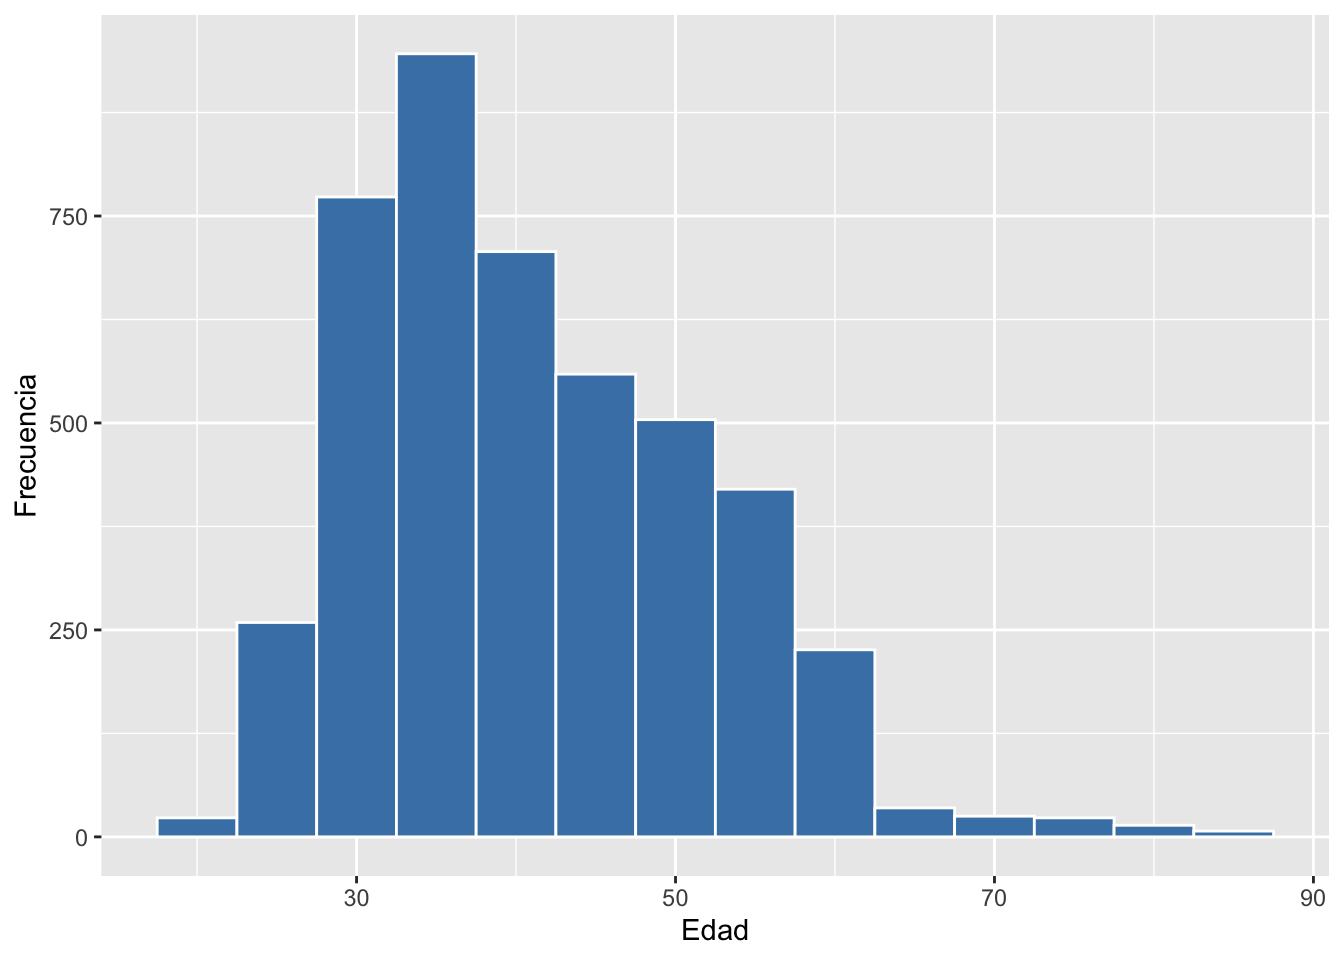
\includegraphics[keepaspectratio]{TP1_files/figure-latex/unnamed-chunk-3-1.pdf}}

\begin{Shaded}
\begin{Highlighting}[]
\CommentTok{\# Comparación de una variable categórica con la variable objetivo}
\FunctionTok{ggplot}\NormalTok{(bank, }\FunctionTok{aes}\NormalTok{(}\AttributeTok{x =}\NormalTok{ job, }\AttributeTok{fill =}\NormalTok{ y)) }\SpecialCharTok{+}
  \FunctionTok{geom\_bar}\NormalTok{(}\AttributeTok{position =} \StringTok{"fill"}\NormalTok{) }\SpecialCharTok{+}
  \FunctionTok{labs}\NormalTok{(}\AttributeTok{title =} \StringTok{"Proporción de aceptación del depósito según ocupación"}\NormalTok{,}
       \AttributeTok{x =} \StringTok{"Ocupación"}\NormalTok{, }\AttributeTok{y =} \StringTok{"Proporción"}\NormalTok{) }\SpecialCharTok{+}
  \FunctionTok{theme}\NormalTok{(}\AttributeTok{axis.text.x =} \FunctionTok{element\_text}\NormalTok{(}\AttributeTok{angle =} \DecValTok{45}\NormalTok{, }\AttributeTok{hjust =} \DecValTok{1}\NormalTok{))}
\end{Highlighting}
\end{Shaded}

\pandocbounded{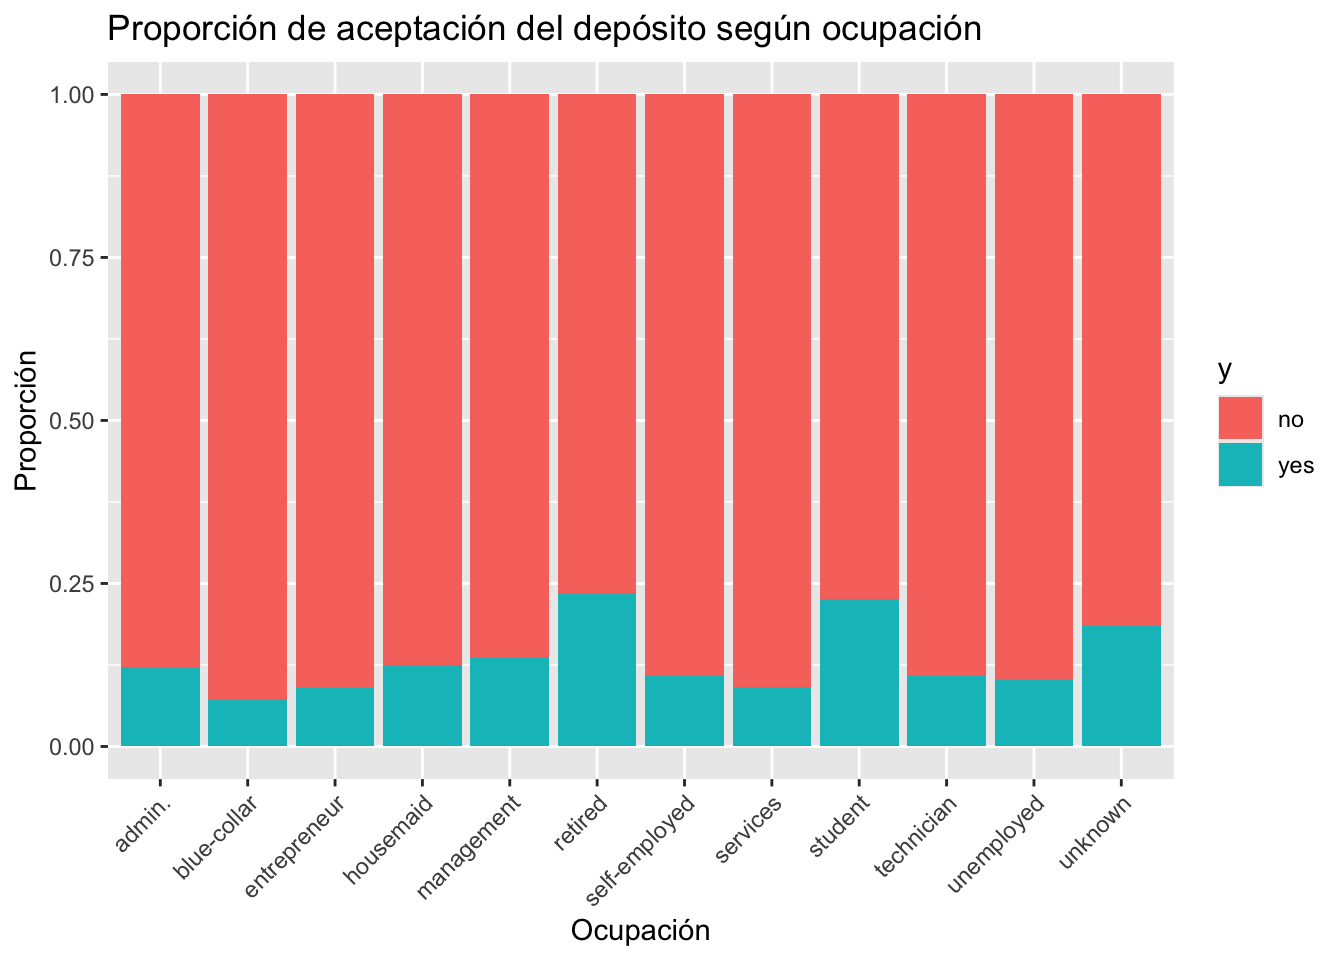
\includegraphics[keepaspectratio]{TP1_files/figure-latex/unnamed-chunk-3-2.pdf}}

\subsubsection{Comentarios sobre los
datos:}\label{comentarios-sobre-los-datos}

\begin{itemize}
\item
  \textbf{Edad}: la mayoría de los clientes se concentran entre los 30 y
  50 años, con algunos outliers en edades más altas.
\item
  \textbf{Ocupación}: existen diferencias notorias en la tasa de
  aceptación de la campaña según el tipo de trabajo; por ejemplo,
  clientes en sectores administrativos tienden a tener una proporción
  distinta a los desempleados o estudiantes.
\item
  \textbf{Balance de cuenta y duración de llamada}: presentan gran
  variabilidad y podrían ser predictores relevantes para el modelo.
\item
  \textbf{Desbalance de clases}: la variable objetivo está desbalanceada
  (muchos más \emph{no} que \emph{sí}), lo cual será importante a
  considerar en la modelización.
\end{itemize}

\subsection{Sección 3: Construcción de un árbol de decisión
básico}\label{secciuxf3n-3-construcciuxf3n-de-un-uxe1rbol-de-decisiuxf3n-buxe1sico}

\begin{Shaded}
\begin{Highlighting}[]
\NormalTok{n }\OtherTok{\textless{}{-}} \FunctionTok{nrow}\NormalTok{(bank)}

\CommentTok{\# límites}
\NormalTok{max\_valid }\OtherTok{\textless{}{-}} \FunctionTok{floor}\NormalTok{(}\FloatTok{0.15} \SpecialCharTok{*}\NormalTok{ n)}
\NormalTok{max\_test  }\OtherTok{\textless{}{-}} \FunctionTok{floor}\NormalTok{(}\FloatTok{0.15} \SpecialCharTok{*}\NormalTok{ n)}

\CommentTok{\# listas de índices}
\NormalTok{idx\_entrenamiento }\OtherTok{\textless{}{-}} \FunctionTok{integer}\NormalTok{(}\DecValTok{0}\NormalTok{)}
\NormalTok{idx\_validacion    }\OtherTok{\textless{}{-}} \FunctionTok{integer}\NormalTok{(}\DecValTok{0}\NormalTok{)}
\NormalTok{idx\_testeo        }\OtherTok{\textless{}{-}} \FunctionTok{integer}\NormalTok{(}\DecValTok{0}\NormalTok{)}

\ControlFlowTok{for}\NormalTok{ (i }\ControlFlowTok{in} \DecValTok{1}\SpecialCharTok{:}\NormalTok{n) \{}
\NormalTok{  r }\OtherTok{\textless{}{-}} \FunctionTok{runif}\NormalTok{(}\DecValTok{1}\NormalTok{)  }\CommentTok{\# número aleatorio entre 0 y 1}

  \ControlFlowTok{if}\NormalTok{ (r }\SpecialCharTok{\textless{}} \FloatTok{0.15} \SpecialCharTok{\&\&} \FunctionTok{length}\NormalTok{(idx\_validacion) }\SpecialCharTok{\textless{}}\NormalTok{ max\_valid) \{}
\NormalTok{    idx\_validacion }\OtherTok{\textless{}{-}} \FunctionTok{c}\NormalTok{(idx\_validacion, i)}
\NormalTok{  \} }\ControlFlowTok{else} \ControlFlowTok{if}\NormalTok{ (r }\SpecialCharTok{\textless{}} \FloatTok{0.30} \SpecialCharTok{\&\&} \FunctionTok{length}\NormalTok{(idx\_testeo) }\SpecialCharTok{\textless{}}\NormalTok{ max\_test) \{}
\NormalTok{    idx\_testeo }\OtherTok{\textless{}{-}} \FunctionTok{c}\NormalTok{(idx\_testeo, i)}
\NormalTok{  \} }\ControlFlowTok{else}\NormalTok{ \{}
\NormalTok{    idx\_entrenamiento }\OtherTok{\textless{}{-}} \FunctionTok{c}\NormalTok{(idx\_entrenamiento, i)}
\NormalTok{  \}}
\NormalTok{\}}

\CommentTok{\# subconjuntos finales}
\NormalTok{entrenamiento }\OtherTok{\textless{}{-}}\NormalTok{ bank[idx\_entrenamiento, , drop }\OtherTok{=} \ConstantTok{FALSE}\NormalTok{]}
\NormalTok{validacion    }\OtherTok{\textless{}{-}}\NormalTok{ bank[idx\_validacion,    , drop }\OtherTok{=} \ConstantTok{FALSE}\NormalTok{]}
\NormalTok{testeo        }\OtherTok{\textless{}{-}}\NormalTok{ bank[idx\_testeo,        , drop }\OtherTok{=} \ConstantTok{FALSE}\NormalTok{]}
\end{Highlighting}
\end{Shaded}

\begin{Shaded}
\begin{Highlighting}[]
\CommentTok{\# Entrenar árbol básico con defaults}
\NormalTok{arbol\_basico }\OtherTok{\textless{}{-}} \FunctionTok{rpart}\NormalTok{(}
\NormalTok{  y }\SpecialCharTok{\textasciitilde{}}\NormalTok{ .,}
  \AttributeTok{data   =}\NormalTok{ entrenamiento,}
  \AttributeTok{method =} \StringTok{"class"}
\NormalTok{)}
\end{Highlighting}
\end{Shaded}

\paragraph{\texorpdfstring{Hiperparámetros por defecto de
\texttt{rpart}}{Hiperparámetros por defecto de rpart}}\label{hiperparuxe1metros-por-defecto-de-rpart}

\begin{itemize}
\item
  \textbf{\texttt{minsplit\ =\ 20}}\strut \\
  Un nodo debe tener \textbf{al menos 20} observaciones para que se
  intente un split. Limita la fragmentación temprana y reduce el
  sobreajuste en nodos muy chicos.
\item
  \textbf{\texttt{minbucket\ =\ round(minsplit/3)} → \textasciitilde7}\\
  Tamaño mínimo de \textbf{cada hoja}. Con el valor por defecto de
  \texttt{minsplit}, cada hoja terminal debe tener \textasciitilde7
  observaciones. Evita hojas ínfimas e inestables.
\item
  \textbf{\texttt{cp\ =\ 0.01}} (complexity parameter)\\
  Solo se aceptan splits que reduzcan el error relativo \textbf{≥ 1\%}.
  Favorece árboles más chicos y acelera el ajuste. Luego se genera la
  secuencia de podas según \texttt{cp}.
\item
  \textbf{\texttt{xval\ =\ 10}}\strut \\
  \textbf{Validación cruzada 10-fold interna} para estimar el error y
  elegir el nivel de poda (en la tabla de \texttt{cp}).
\item
  \textbf{\texttt{maxdepth\ =\ 30}}\strut \\
  Profundidad máxima muy alta (prácticamente sin tope en la práctica).
  El control real de complejidad lo imponen \texttt{cp},
  \texttt{minsplit} y \texttt{minbucket}.
\item
  \textbf{\texttt{maxcompete\ =\ 4}}\strut \\
  Guarda hasta \textbf{4 splits competidores} por nodo (no afecta el
  ajuste; es metadato útil para inspección).
\item
  \textbf{\texttt{maxsurrogate\ =\ 5}}\strut \\
  Guarda hasta \textbf{5 variables sustitutas} por nodo para manejar
  \textbf{valores faltantes}.
\item
  \textbf{\texttt{usesurrogate\ =\ 2}}\strut \\
  Si falta la variable del split principal, \textbf{usa surrogates en
  orden}; si tampoco están disponibles, envía el caso por la
  \textbf{rama mayoritaria}.
\item
  \textbf{\texttt{surrogatestyle\ =\ 0}}\strut \\
  El ``mejor'' surrogate se elige por \textbf{número total de aciertos}
  (penaliza variables con muchos NA).
\item
  (\textbf{Clasificación}) \textbf{\texttt{split\ =\ "gini"}},
  \textbf{\texttt{prior}} proporcionales a las \textbf{frecuencias de
  clase observadas} y \textbf{\texttt{loss}} con costo uniforme de error
  (0 en la diagonal y 1 fuera de la diagonal).\\
  Implica que los cortes minimizan \textbf{impureza Gini}, asumiendo las
  prevalencias del dataset y costos de clasificación iguales, salvo que
  se especifiquen otros.
\end{itemize}

\begin{Shaded}
\begin{Highlighting}[]
\FunctionTok{library}\NormalTok{(rpart.plot)}
\CommentTok{\# Visualización}
\FunctionTok{rpart.plot}\NormalTok{(arbol\_basico, }\AttributeTok{type =} \DecValTok{2}\NormalTok{, }\AttributeTok{extra =} \DecValTok{106}\NormalTok{, }\AttributeTok{box.palette =} \StringTok{"GnBu"}\NormalTok{)}
\end{Highlighting}
\end{Shaded}

\pandocbounded{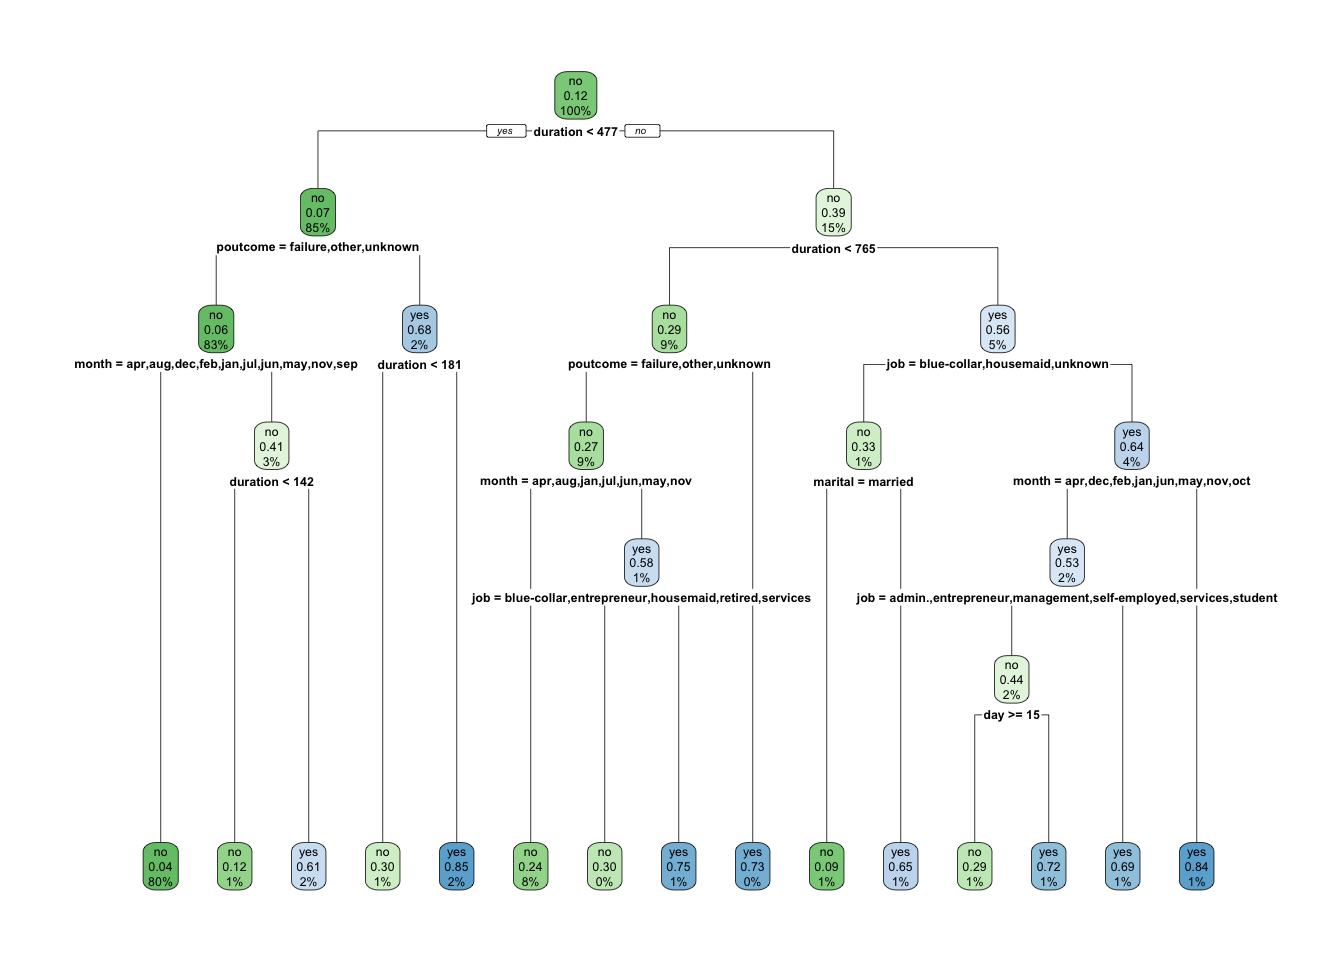
\includegraphics[keepaspectratio]{TP1_files/figure-latex/unnamed-chunk-6-1.pdf}}

\textbf{Altura observada:} 5 niveles (raíz + 4 divisiones).

\begin{enumerate}
\def\labelenumi{\arabic{enumi})}
\item
  \textbf{Raíz --- \texttt{duration\ \textless{}\ 477\ s}}\\
  Divide ``llamadas cortas'' vs ``largas''. Es el corte más informativo:
  las cortas concentran \textbf{NO}, las largas elevan la chance de
  \textbf{YES}.
\item
  \textbf{Rama izquierda (\texttt{duration\ \textless{}\ 477})}

  \begin{itemize}
  \tightlist
  \item
    Siguientes cortes: \textbf{\texttt{poutcome}} (resultados previos de
    campaña), \textbf{\texttt{month}} y umbrales más bajos de
    \textbf{\texttt{duration}} (≈ 180 s).\\
  \item
    Interpretación: \textbf{llamadas muy cortas} y \textbf{sin buen
    antecedente} tienden a \textbf{NO}. Los ajustes con \texttt{month}
    refinan pequeños subgrupos.
  \end{itemize}
\item
  \textbf{Rama derecha (\texttt{duration\ ≥\ 477})}

  \begin{itemize}
  \tightlist
  \item
    Segundo umbral de \textbf{\texttt{duration}}: \textbf{≈ 765 s}
    separa \textbf{llamadas largas} (alta probabilidad de \textbf{YES})
    de las \textbf{intermedias}.\\
  \item
    En la franja intermedia, la decisión se afina con
    \textbf{\texttt{job}}, \textbf{\texttt{marital}}, y en menor medida
    \textbf{\texttt{month/day}}:

    \begin{itemize}
    \tightlist
    \item
      Ocupaciones no profesionales y \texttt{marital\ =\ married}
      empujan a \textbf{NO}.\\
    \item
      Ocupaciones profesionales/servicios y otros estados civiles elevan
      la chance de \textbf{YES}.
    \end{itemize}
  \end{itemize}
\end{enumerate}

\subsection{4. Evaluación del árbol de decisión
básico}\label{evaluaciuxf3n-del-uxe1rbol-de-decisiuxf3n-buxe1sico}

\begin{Shaded}
\begin{Highlighting}[]
\CommentTok{\# Normalización de niveles en los tres splits}
\ControlFlowTok{for}\NormalTok{ (nm }\ControlFlowTok{in} \FunctionTok{c}\NormalTok{(}\StringTok{"entrenamiento"}\NormalTok{, }\StringTok{"validacion"}\NormalTok{, }\StringTok{"testeo"}\NormalTok{)) \{}
  \ControlFlowTok{if}\NormalTok{ (}\FunctionTok{exists}\NormalTok{(nm)) \{}
\NormalTok{    tmp }\OtherTok{\textless{}{-}} \FunctionTok{get}\NormalTok{(nm)}
    \ControlFlowTok{if}\NormalTok{ (}\SpecialCharTok{!}\FunctionTok{is.factor}\NormalTok{(tmp}\SpecialCharTok{$}\NormalTok{y)) tmp}\SpecialCharTok{$}\NormalTok{y }\OtherTok{\textless{}{-}} \FunctionTok{as.factor}\NormalTok{(tmp}\SpecialCharTok{$}\NormalTok{y)}
    \ControlFlowTok{if}\NormalTok{ (}\FunctionTok{all}\NormalTok{(}\FunctionTok{c}\NormalTok{(}\StringTok{"no"}\NormalTok{, }\StringTok{"yes"}\NormalTok{) }\SpecialCharTok{\%in\%} \FunctionTok{levels}\NormalTok{(tmp}\SpecialCharTok{$}\NormalTok{y))) \{}
\NormalTok{      tmp}\SpecialCharTok{$}\NormalTok{y }\OtherTok{\textless{}{-}} \FunctionTok{factor}\NormalTok{(tmp}\SpecialCharTok{$}\NormalTok{y, }\AttributeTok{levels =} \FunctionTok{c}\NormalTok{(}\StringTok{"no"}\NormalTok{, }\StringTok{"yes"}\NormalTok{))}
\NormalTok{    \}}
    \FunctionTok{assign}\NormalTok{(nm, tmp)}
\NormalTok{  \}}
\NormalTok{\}}

\CommentTok{\# Chequeos}
\FunctionTok{stopifnot}\NormalTok{(}\FunctionTok{exists}\NormalTok{(}\StringTok{"arbol\_basico"}\NormalTok{), }\FunctionTok{exists}\NormalTok{(}\StringTok{"testeo"}\NormalTok{))}
\FunctionTok{stopifnot}\NormalTok{(}\StringTok{"y"} \SpecialCharTok{\%in\%} \FunctionTok{names}\NormalTok{(testeo))}
\FunctionTok{stopifnot}\NormalTok{(}\FunctionTok{is.factor}\NormalTok{(testeo}\SpecialCharTok{$}\NormalTok{y))}

\CommentTok{\# Predicciones en testeo}
\NormalTok{pred\_class }\OtherTok{\textless{}{-}} \FunctionTok{predict}\NormalTok{(arbol\_basico, }\AttributeTok{newdata =}\NormalTok{ testeo, }\AttributeTok{type =} \StringTok{"class"}\NormalTok{)}
\NormalTok{pred\_class }\OtherTok{\textless{}{-}} \FunctionTok{factor}\NormalTok{(pred\_class, }\AttributeTok{levels =} \FunctionTok{levels}\NormalTok{(testeo}\SpecialCharTok{$}\NormalTok{y))}

\NormalTok{pred\_prob\_mat }\OtherTok{\textless{}{-}} \FunctionTok{predict}\NormalTok{(arbol\_basico, }\AttributeTok{newdata =}\NormalTok{ testeo, }\AttributeTok{type =} \StringTok{"prob"}\NormalTok{)}
\NormalTok{pos\_col }\OtherTok{\textless{}{-}} \ControlFlowTok{if}\NormalTok{ (}\StringTok{"yes"} \SpecialCharTok{\%in\%} \FunctionTok{colnames}\NormalTok{(pred\_prob\_mat)) }\StringTok{"yes"} \ControlFlowTok{else} \FunctionTok{tail}\NormalTok{(}\FunctionTok{colnames}\NormalTok{(pred\_prob\_mat), }\DecValTok{1}\NormalTok{)}
\NormalTok{pred\_prob }\OtherTok{\textless{}{-}}\NormalTok{ pred\_prob\_mat[, pos\_col]}

\CommentTok{\# Matriz de confusión y métricas}
\NormalTok{matriz\_conf }\OtherTok{\textless{}{-}}\NormalTok{ caret}\SpecialCharTok{::}\FunctionTok{confusionMatrix}\NormalTok{(pred\_class, testeo}\SpecialCharTok{$}\NormalTok{y, }\AttributeTok{positive =} \StringTok{"yes"}\NormalTok{)}

\NormalTok{accuracy  }\OtherTok{\textless{}{-}}\NormalTok{ matriz\_conf}\SpecialCharTok{$}\NormalTok{overall[}\StringTok{"Accuracy"}\NormalTok{]}
\NormalTok{precision }\OtherTok{\textless{}{-}}\NormalTok{ matriz\_conf}\SpecialCharTok{$}\NormalTok{byClass[}\StringTok{"Precision"}\NormalTok{]}
\NormalTok{recall    }\OtherTok{\textless{}{-}}\NormalTok{ matriz\_conf}\SpecialCharTok{$}\NormalTok{byClass[}\StringTok{"Recall"}\NormalTok{]}
\NormalTok{f1        }\OtherTok{\textless{}{-}}\NormalTok{ matriz\_conf}\SpecialCharTok{$}\NormalTok{byClass[}\StringTok{"F1"}\NormalTok{]}

\CommentTok{\# {-}{-}{-} Gráficos: Matriz de confusión (conteos y proporciones) {-}{-}{-}{-}{-}{-}{-}{-}{-}{-}{-}{-}{-}{-}{-}{-}{-}{-}}

\CommentTok{\# Conteos}
\NormalTok{cm\_tbl }\OtherTok{\textless{}{-}} \FunctionTok{as.table}\NormalTok{(matriz\_conf}\SpecialCharTok{$}\NormalTok{table)}
\NormalTok{cm\_df }\OtherTok{\textless{}{-}} \FunctionTok{as.data.frame}\NormalTok{(cm\_tbl)}
\FunctionTok{names}\NormalTok{(cm\_df) }\OtherTok{\textless{}{-}} \FunctionTok{c}\NormalTok{(}\StringTok{"real"}\NormalTok{, }\StringTok{"pred"}\NormalTok{, }\StringTok{"freq"}\NormalTok{)}

\FunctionTok{ggplot}\NormalTok{(cm\_df, }\FunctionTok{aes}\NormalTok{(}\AttributeTok{x =}\NormalTok{ real, }\AttributeTok{y =}\NormalTok{ pred, }\AttributeTok{fill =}\NormalTok{ freq)) }\SpecialCharTok{+}
  \FunctionTok{geom\_tile}\NormalTok{(}\AttributeTok{color =} \StringTok{"white"}\NormalTok{) }\SpecialCharTok{+}
  \FunctionTok{geom\_text}\NormalTok{(}\FunctionTok{aes}\NormalTok{(}\AttributeTok{label =}\NormalTok{ freq), }\AttributeTok{size =} \DecValTok{4}\NormalTok{) }\SpecialCharTok{+}
  \FunctionTok{scale\_fill\_gradient}\NormalTok{(}\AttributeTok{low =} \StringTok{"lightblue"}\NormalTok{, }\AttributeTok{high =} \StringTok{"steelblue"}\NormalTok{) }\SpecialCharTok{+}
  \FunctionTok{labs}\NormalTok{(}
    \AttributeTok{title =} \StringTok{"Matriz de confusión (conteos)"}\NormalTok{,}
    \AttributeTok{x =} \StringTok{"Valor real"}\NormalTok{,}
    \AttributeTok{y =} \StringTok{"Predicción"}\NormalTok{,}
    \AttributeTok{fill =} \StringTok{"Frecuencia"}
\NormalTok{  ) }\SpecialCharTok{+}
  \FunctionTok{theme\_minimal}\NormalTok{()}
\end{Highlighting}
\end{Shaded}

\pandocbounded{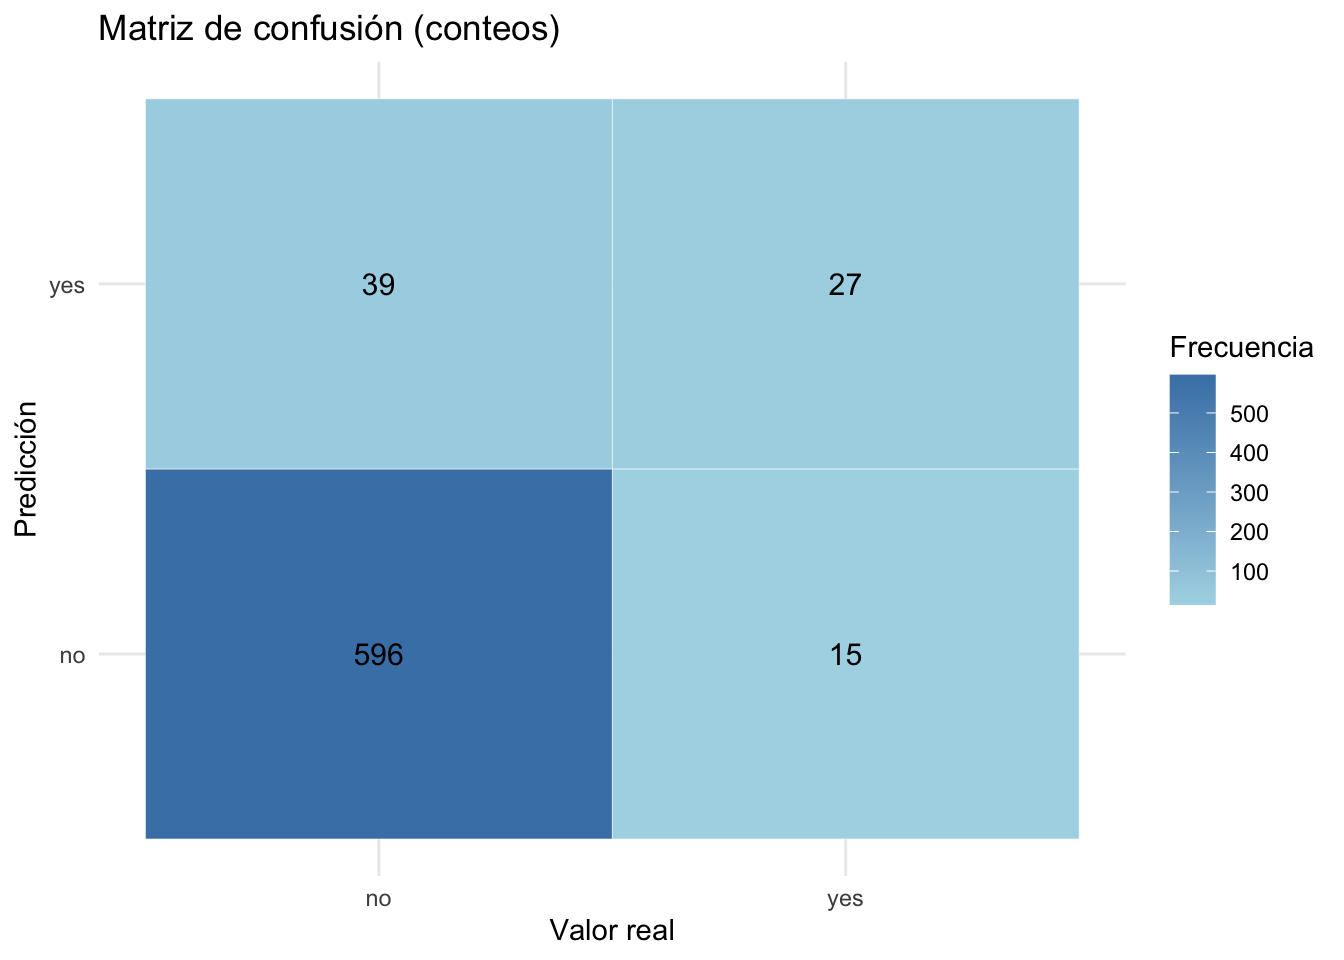
\includegraphics[keepaspectratio]{TP1_files/figure-latex/unnamed-chunk-7-1.pdf}}

\begin{Shaded}
\begin{Highlighting}[]
\CommentTok{\# Proporciones por clase real}
\NormalTok{cm\_prop }\OtherTok{\textless{}{-}}\NormalTok{ dplyr}\SpecialCharTok{::}\FunctionTok{group\_by}\NormalTok{(cm\_df, real)}
\NormalTok{cm\_prop }\OtherTok{\textless{}{-}}\NormalTok{ dplyr}\SpecialCharTok{::}\FunctionTok{mutate}\NormalTok{(cm\_prop, }\AttributeTok{prop =}\NormalTok{ freq }\SpecialCharTok{/} \FunctionTok{sum}\NormalTok{(freq))}
\NormalTok{cm\_prop }\OtherTok{\textless{}{-}}\NormalTok{ dplyr}\SpecialCharTok{::}\FunctionTok{ungroup}\NormalTok{(cm\_prop)}

\FunctionTok{ggplot}\NormalTok{(cm\_prop, }\FunctionTok{aes}\NormalTok{(}\AttributeTok{x =}\NormalTok{ real, }\AttributeTok{y =}\NormalTok{ pred, }\AttributeTok{fill =}\NormalTok{ prop)) }\SpecialCharTok{+}
  \FunctionTok{geom\_tile}\NormalTok{(}\AttributeTok{color =} \StringTok{"white"}\NormalTok{) }\SpecialCharTok{+}
  \FunctionTok{geom\_text}\NormalTok{(}\FunctionTok{aes}\NormalTok{(}\AttributeTok{label =} \FunctionTok{sprintf}\NormalTok{(}\StringTok{"\%.1f\%\%"}\NormalTok{, }\DecValTok{100} \SpecialCharTok{*}\NormalTok{ prop)), }\AttributeTok{size =} \DecValTok{4}\NormalTok{) }\SpecialCharTok{+}
  \FunctionTok{scale\_fill\_gradient}\NormalTok{(}\AttributeTok{low =} \StringTok{"lavender"}\NormalTok{, }\AttributeTok{high =} \StringTok{"purple"}\NormalTok{) }\SpecialCharTok{+}
  \FunctionTok{labs}\NormalTok{(}
    \AttributeTok{title =} \StringTok{"Matriz de confusión (proporciones por real)"}\NormalTok{,}
    \AttributeTok{x =} \StringTok{"Valor real"}\NormalTok{,}
    \AttributeTok{y =} \StringTok{"Predicción"}\NormalTok{,}
    \AttributeTok{fill =} \StringTok{"Proporción"}
\NormalTok{  ) }\SpecialCharTok{+}
  \FunctionTok{theme\_minimal}\NormalTok{()}
\end{Highlighting}
\end{Shaded}

\pandocbounded{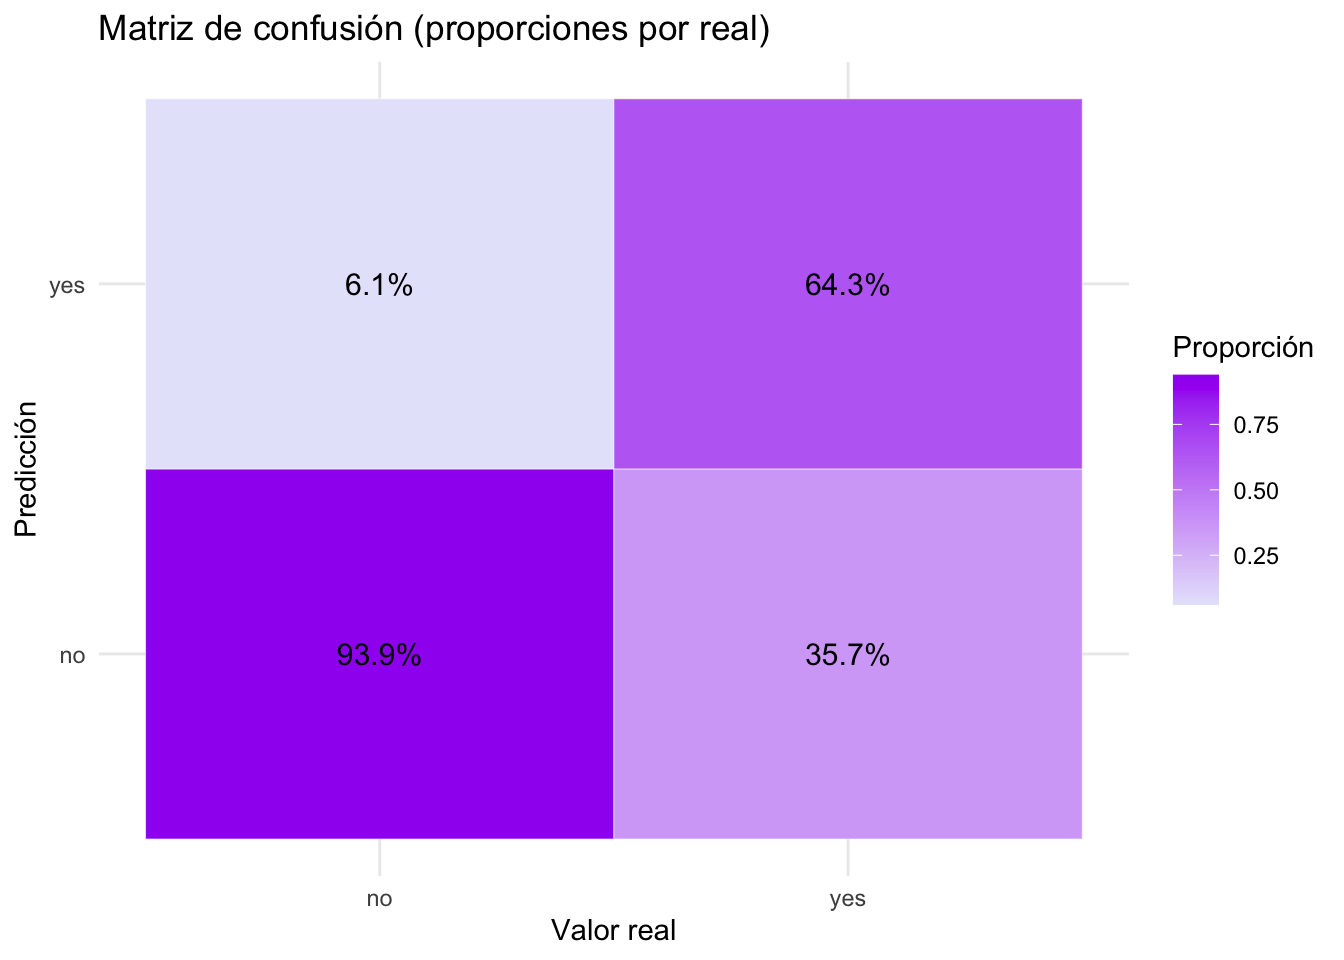
\includegraphics[keepaspectratio]{TP1_files/figure-latex/unnamed-chunk-7-2.pdf}}

\begin{Shaded}
\begin{Highlighting}[]
\CommentTok{\# ROC y AUC}
\NormalTok{roc\_curve }\OtherTok{\textless{}{-}}\NormalTok{ pROC}\SpecialCharTok{::}\FunctionTok{roc}\NormalTok{(}
\NormalTok{  testeo}\SpecialCharTok{$}\NormalTok{y,}
\NormalTok{  pred\_prob,}
  \AttributeTok{levels =} \FunctionTok{c}\NormalTok{(}\StringTok{"no"}\NormalTok{, }\StringTok{"yes"}\NormalTok{),}
  \AttributeTok{direction =} \StringTok{"\textless{}"}
\NormalTok{)}
\NormalTok{auc\_value }\OtherTok{\textless{}{-}}\NormalTok{ pROC}\SpecialCharTok{::}\FunctionTok{auc}\NormalTok{(roc\_curve)}

\CommentTok{\# Tabla resumen}
\NormalTok{resumen }\OtherTok{\textless{}{-}} \FunctionTok{data.frame}\NormalTok{(}
  \AttributeTok{Metrica =} \FunctionTok{c}\NormalTok{(}\StringTok{"Accuracy"}\NormalTok{, }\StringTok{"Precision"}\NormalTok{, }\StringTok{"Recall"}\NormalTok{, }\StringTok{"F1"}\NormalTok{, }\StringTok{"AUC{-}ROC"}\NormalTok{),}
  \AttributeTok{Valor   =} \FunctionTok{c}\NormalTok{(}
    \FunctionTok{as.numeric}\NormalTok{(accuracy),}
    \FunctionTok{as.numeric}\NormalTok{(precision),}
    \FunctionTok{as.numeric}\NormalTok{(recall),}
    \FunctionTok{as.numeric}\NormalTok{(f1),}
    \FunctionTok{as.numeric}\NormalTok{(auc\_value)}
\NormalTok{  )}
\NormalTok{)}
\NormalTok{knitr}\SpecialCharTok{::}\FunctionTok{kable}\NormalTok{(resumen, }\AttributeTok{digits =} \DecValTok{4}\NormalTok{, }\AttributeTok{caption =} \StringTok{"Punto 4 — Métricas (Test)"}\NormalTok{)}
\end{Highlighting}
\end{Shaded}

\begin{longtable}[]{@{}lr@{}}
\caption{Punto 4 --- Métricas (Test)}\tabularnewline
\toprule\noalign{}
Metrica & Valor \\
\midrule\noalign{}
\endfirsthead
\toprule\noalign{}
Metrica & Valor \\
\midrule\noalign{}
\endhead
\bottomrule\noalign{}
\endlastfoot
Accuracy & 0.9202 \\
Precision & 0.6429 \\
Recall & 0.4091 \\
F1 & 0.5000 \\
AUC-ROC & 0.7857 \\
\end{longtable}

\begin{Shaded}
\begin{Highlighting}[]
\FunctionTok{plot}\NormalTok{(roc\_curve, }\AttributeTok{lwd =} \DecValTok{2}\NormalTok{, }\AttributeTok{main =} \StringTok{"Curva ROC — Árbol básico (Test)"}\NormalTok{)}
\FunctionTok{abline}\NormalTok{(}\AttributeTok{a =} \DecValTok{0}\NormalTok{, }\AttributeTok{b =} \DecValTok{1}\NormalTok{, }\AttributeTok{lty =} \DecValTok{2}\NormalTok{)}
\end{Highlighting}
\end{Shaded}

\pandocbounded{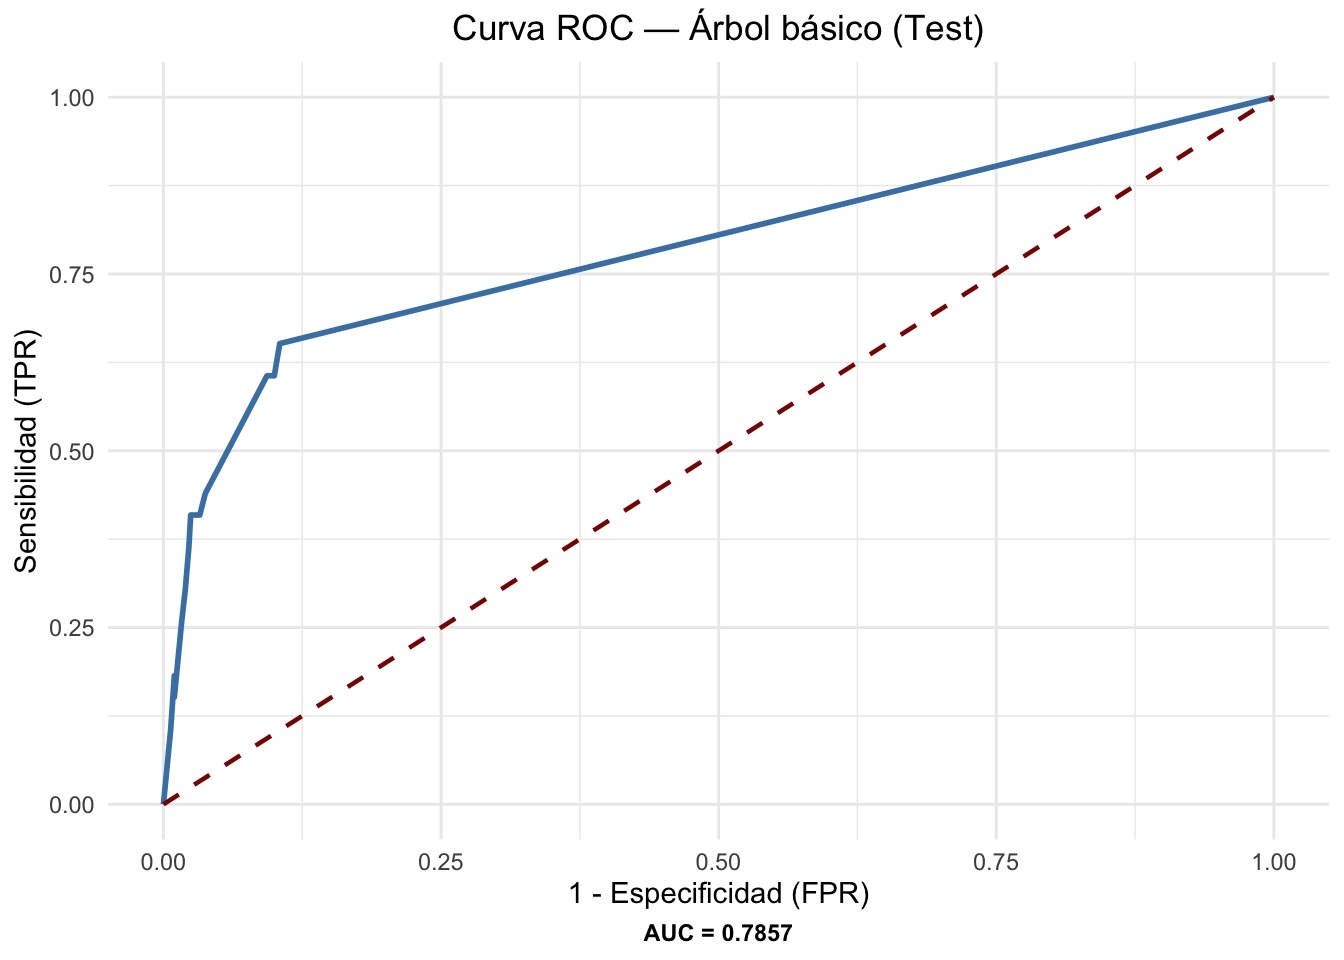
\includegraphics[keepaspectratio]{TP1_files/figure-latex/unnamed-chunk-7-3.pdf}}

\subsubsection{Interpretación de
resultados}\label{interpretaciuxf3n-de-resultados}

Al evaluar el árbol de decisión básico en el conjunto de testeo se
observa que el modelo alcanza un \textbf{accuracy de aproximadamente
92\%}, un valor elevado y aparentemente satisfactorio a primera vista.
Sin embargo, al analizar con mayor detalle la matriz de confusión se
advierte que este buen desempeño global está muy influido por el
\textbf{desbalance de clases}: la mayoría de los clientes pertenece a la
clase negativa (``no''), por lo que un modelo que siempre predijera
``no'' alcanzaría un \textbf{No Information Rate (NIR) del 90\%}. Esto
significa que la mejora real sobre una estrategia trivial es más
reducida de lo que sugiere el valor bruto del accuracy, e incluso la
prueba de significancia muestra que la diferencia respecto al NIR no es
concluyente al 5\% de significancia.

La interpretación cambia si se examinan otras métricas específicas de la
clase positiva. La \textbf{precisión (precision)} alcanza un 64\%, lo
que indica que cuando el modelo se arriesga a predecir que un cliente
aceptará el depósito (``yes''), tiene más de la mitad de probabilidades
de estar en lo cierto. Sin embargo, la \textbf{sensibilidad (recall)} es
mucho más baja, alrededor de 41\%, lo que significa que el árbol deja
escapar a más de la mitad de los clientes que efectivamente aceptan la
oferta. Esto se traduce en un número importante de falsos negativos (39
en el testeo), lo que podría ser problemático en un contexto de
marketing donde detectar a los posibles clientes interesados suele ser
más importante que evitar falsos positivos. El \textbf{F1-score}, que
combina precisión y recall en una sola medida, queda en torno a 0.50, lo
que confirma un equilibrio modesto y refleja la dificultad del modelo
para captar de manera consistente la clase minoritaria.

En contraste, la \textbf{especificidad del modelo es muy alta (97.5\%)},
lo cual significa que el árbol distingue muy bien a los clientes que no
contratarán el depósito, cometiendo muy pocos falsos positivos. Esta
asimetría entre sensibilidad y especificidad está en línea con lo que se
observa en la prueba de McNemar, que arroja un p-valor significativo
indicando que los errores no se distribuyen de manera balanceada: el
modelo tiende claramente a equivocarse más en los positivos que en los
negativos.

Finalmente, la \textbf{curva ROC y el AUC confirman la existencia de
señal predictiva}. El área bajo la curva se ubica en 0.79, lo que indica
que, si se toma al azar un cliente que aceptó y uno que rechazó la
oferta, en casi ocho de cada diez casos el modelo asigna una
probabilidad mayor al cliente positivo que al negativo. Este valor
refleja que, más allá del umbral de decisión fijo que usa \texttt{rpart}
(basado en la mayoría de la hoja, equivalente a 0.5), las probabilidades
generadas contienen información útil y podrían aprovecharse para mejorar
el recall ajustando el umbral de clasificación.

\end{document}
